\section{Introduction}

\subsection{RoboJackets}

%stuff about club and teams
RoboJackets is an robotics competition and outreach group that has been operating at the Georgia Institute of Technology since 1999. Overall the RoboJackets consist of four teams a FIRST outreach / mentorship, Middle Weight BattleBots, RoboCup Small Size and IGVC. In all members come from many of the engineering departments across campus (prominently Mechanical, Aerospace, Electrical, and Computer Science) thus providing a truly multidisciplinary robotics development experience. The RoboJackets IGVC Team initially started in 2004 has fielded a team every year except 2005 and has been able to attain a top ten finish in the autonomous course since 2007. This past January, the RoboJackets along with the entire Student Competition Center moved to a new off campus facility. The move in total represented a loss of nearly two months of work, but given this many upgrades were still undertaken. 

\subsection{Team Members}

The 2011 team members are listed in Table \ref{TAB:RJTeam}.

\begin{table}[H]
\begin{center}
\caption{2011 RoboJackets / IGVC Team}
\begin{tabular}{| l | p{2.4in} | p{2in} |}
\hline
Name & Degree / Class & Role\\ \hline
Joe Hickey &		BS Mechanical Engineering / Sophomore&	Mechanical design and build\\ \hline
John Madden &		BS Mechanical Engineering and Computer Science/ Senior & Project Manager, Mechanical build, Software\\ \hline
Kenneth Marino &	BS Electrical Engineering / Sophomore&	Software, Electronics\\ \hline
Stefan Posey &		BS Aerospace Engineering / Senior &		Mechanical build\\ \hline
Jacob Schloss &		BS Aerospace Engineering / Senior&	Software, Electronics\\ \hline
Akshay Srivastava &	BS Aerospace Engineering / Junior&	Electronics\\ \hline

\end{tabular}
\label{TAB:RJTeam}
\end{center}
\end{table}

\subsection{Past Competitions}

\begin{figure}[H]
\begin{minipage}[b]{0.5\linewidth}
\centering
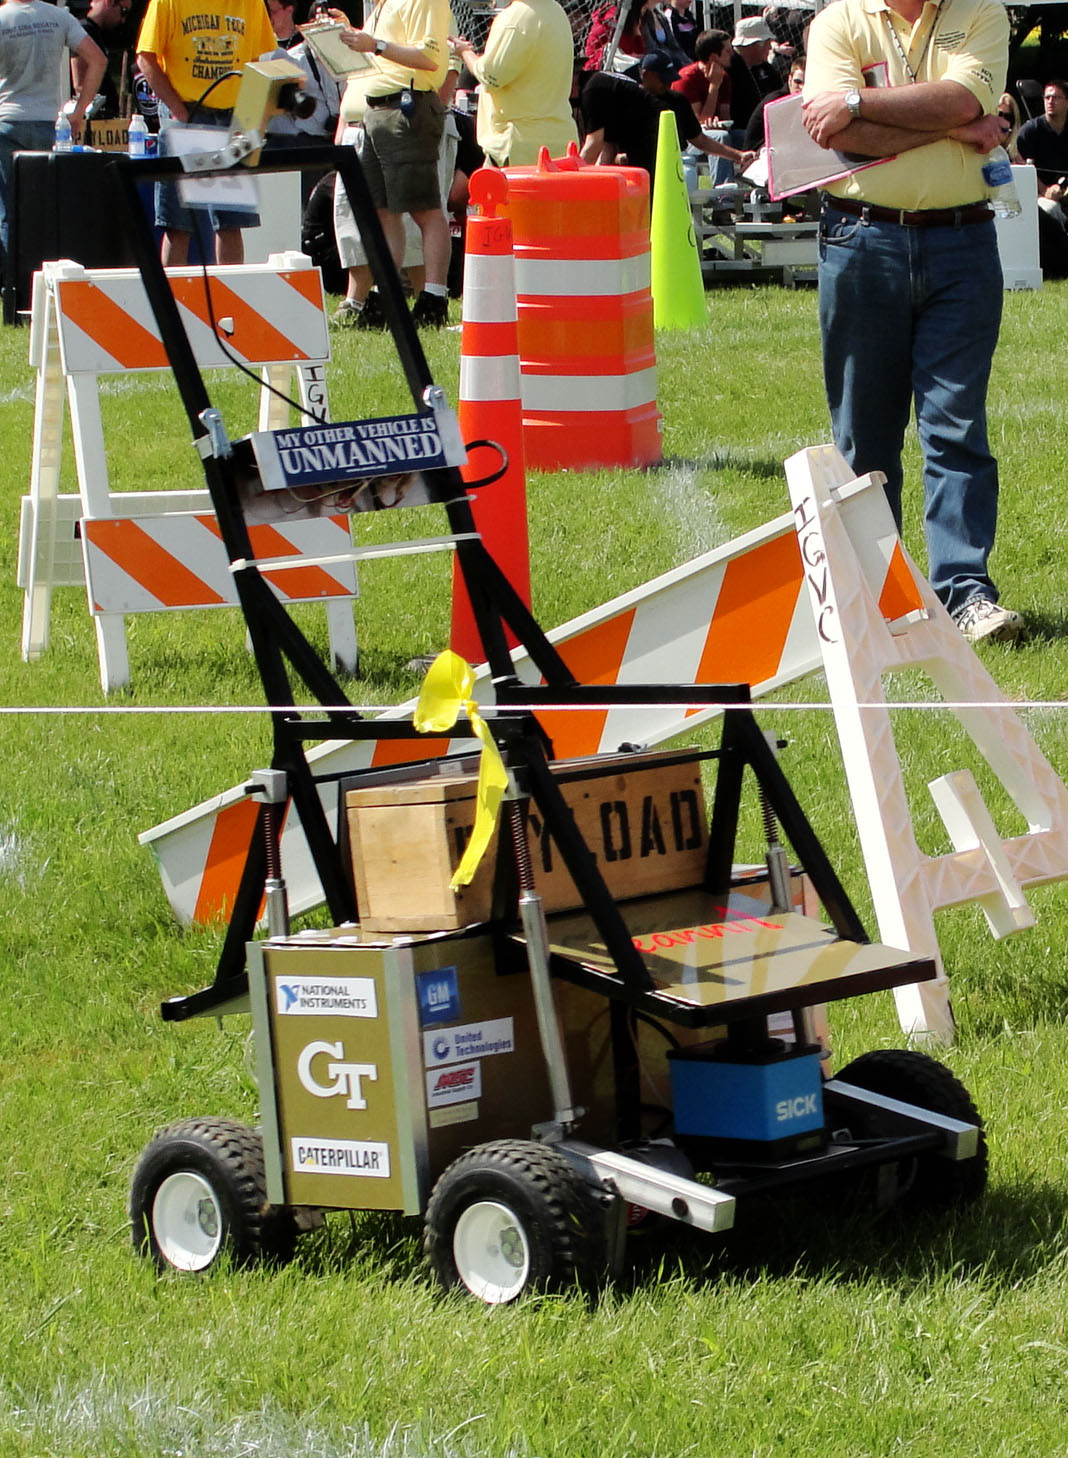
\includegraphics[width=2.5in]{./pics/2010Jeanni.jpg}
\caption{Jeanni, the 2010 base}
\label{FIG:Jeanni}
\end{minipage}
\hspace{0.1in}
\begin{minipage}[b]{0.5\linewidth}
\centering
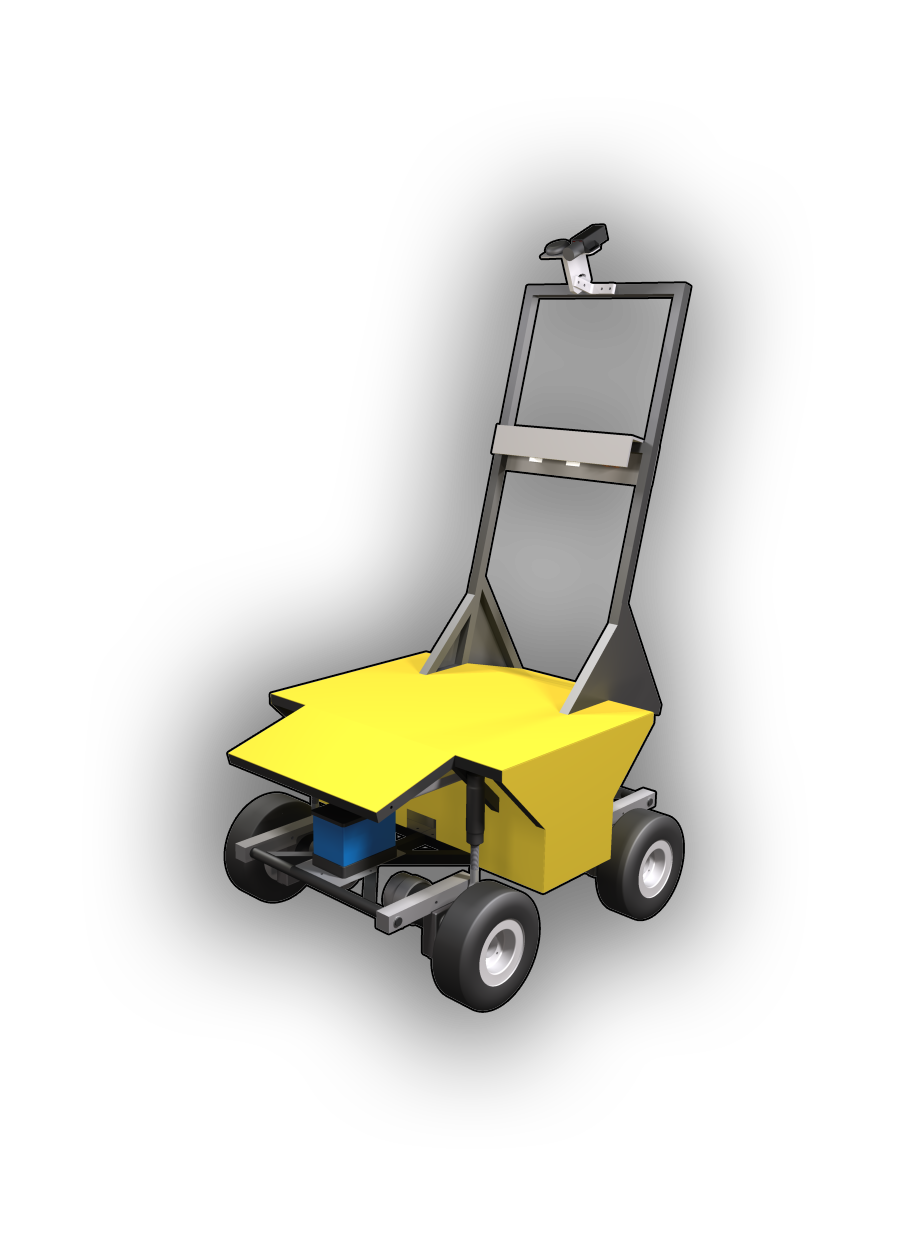
\includegraphics[width=3in]{./pics/RobotFrontCover.png}
\caption{Roxi, the 2011 Base}
\label{FIG:Trans}
\end{minipage}
\end{figure}
